\documentclass[12pt]{article}
\usepackage[a4paper,margin=1in]{geometry}
\usepackage{booktabs}
\usepackage{graphicx}
\usepackage{float}
\usepackage{hyperref}
\usepackage{longtable}
\usepackage{array}
\usepackage{caption}

\title{Armenia Labour Force Survey (2021--2024): Enhanced Statistical Report}
\author{Prepared with the reproducible Python pipeline}
\date{\today}

\begin{document}
\maketitle
\tableofcontents
\newpage

\section{Introduction}
This report evaluates labour-market patterns in Armenia using Armstat Labour Force Survey microdata for 2021--2024. The analysis separates 2024 and compares it with pooled 2021--2023 to highlight potential post-period shifts.

\subsection*{Research Questions}
\begin{enumerate}
    \item Does sectoral employment distribution (agriculture/industry/services) differ by gender and by region?
    \item Is disability status associated with labour-force status (employed/unemployed/out of labour force)?
    \item Among employed workers, does marital status affect monthly income?
    \item Among employed workers, do age groups differ in paid weekly working hours?
    \item Among employed workers, is unpaid domestic work associated with paid working hours?
\end{enumerate}

\section{Data and Processing Workflow}
\subsection{Input data}
Four annual resident files are used: 2021, 2022, 2023, and 2024 Labour Force Survey datasets.

\subsection{Pipeline outputs}
All outputs are automatically generated by \texttt{src/lfs\_analysis.py}:
\begin{itemize}
    \item Main outputs: \texttt{outputs/tables}, \texttt{outputs/figures}, \texttt{outputs/data}
    \item Compatibility mirror (for legacy paths): \texttt{Outputs/tables}, \texttt{Outputs/figures}
\end{itemize}

\subsection{Cleaning and harmonization}
The script harmonizes annual column names using a variable map, replaces questionnaire special codes with missing values, constrains invalid income/hours values, and recodes analytic categories (gender, disability, employment status, marital status, sector, and age groups).

\section{Methods}
\begin{itemize}
    \item \textbf{Chi-square tests}: sector vs gender/region; disability status vs labour-force status.
    \item \textbf{ANOVA}: monthly income by marital status; paid weekly hours by age group.
    \item \textbf{Regression}: paid hours on unpaid domestic work (simple and adjusted with age, gender, marital status).
    \item \textbf{Visualization}: proportion charts, distribution plots, and confidence-interval plots for clearer interpretation.
\end{itemize}

\section{Results and Figures}

\subsection{Q1: Sector by Gender and Region}
Tables: \texttt{outputs/tables/q1\_chi2\_summary.csv}, crosstab exports.

\begin{figure}[H]
\centering
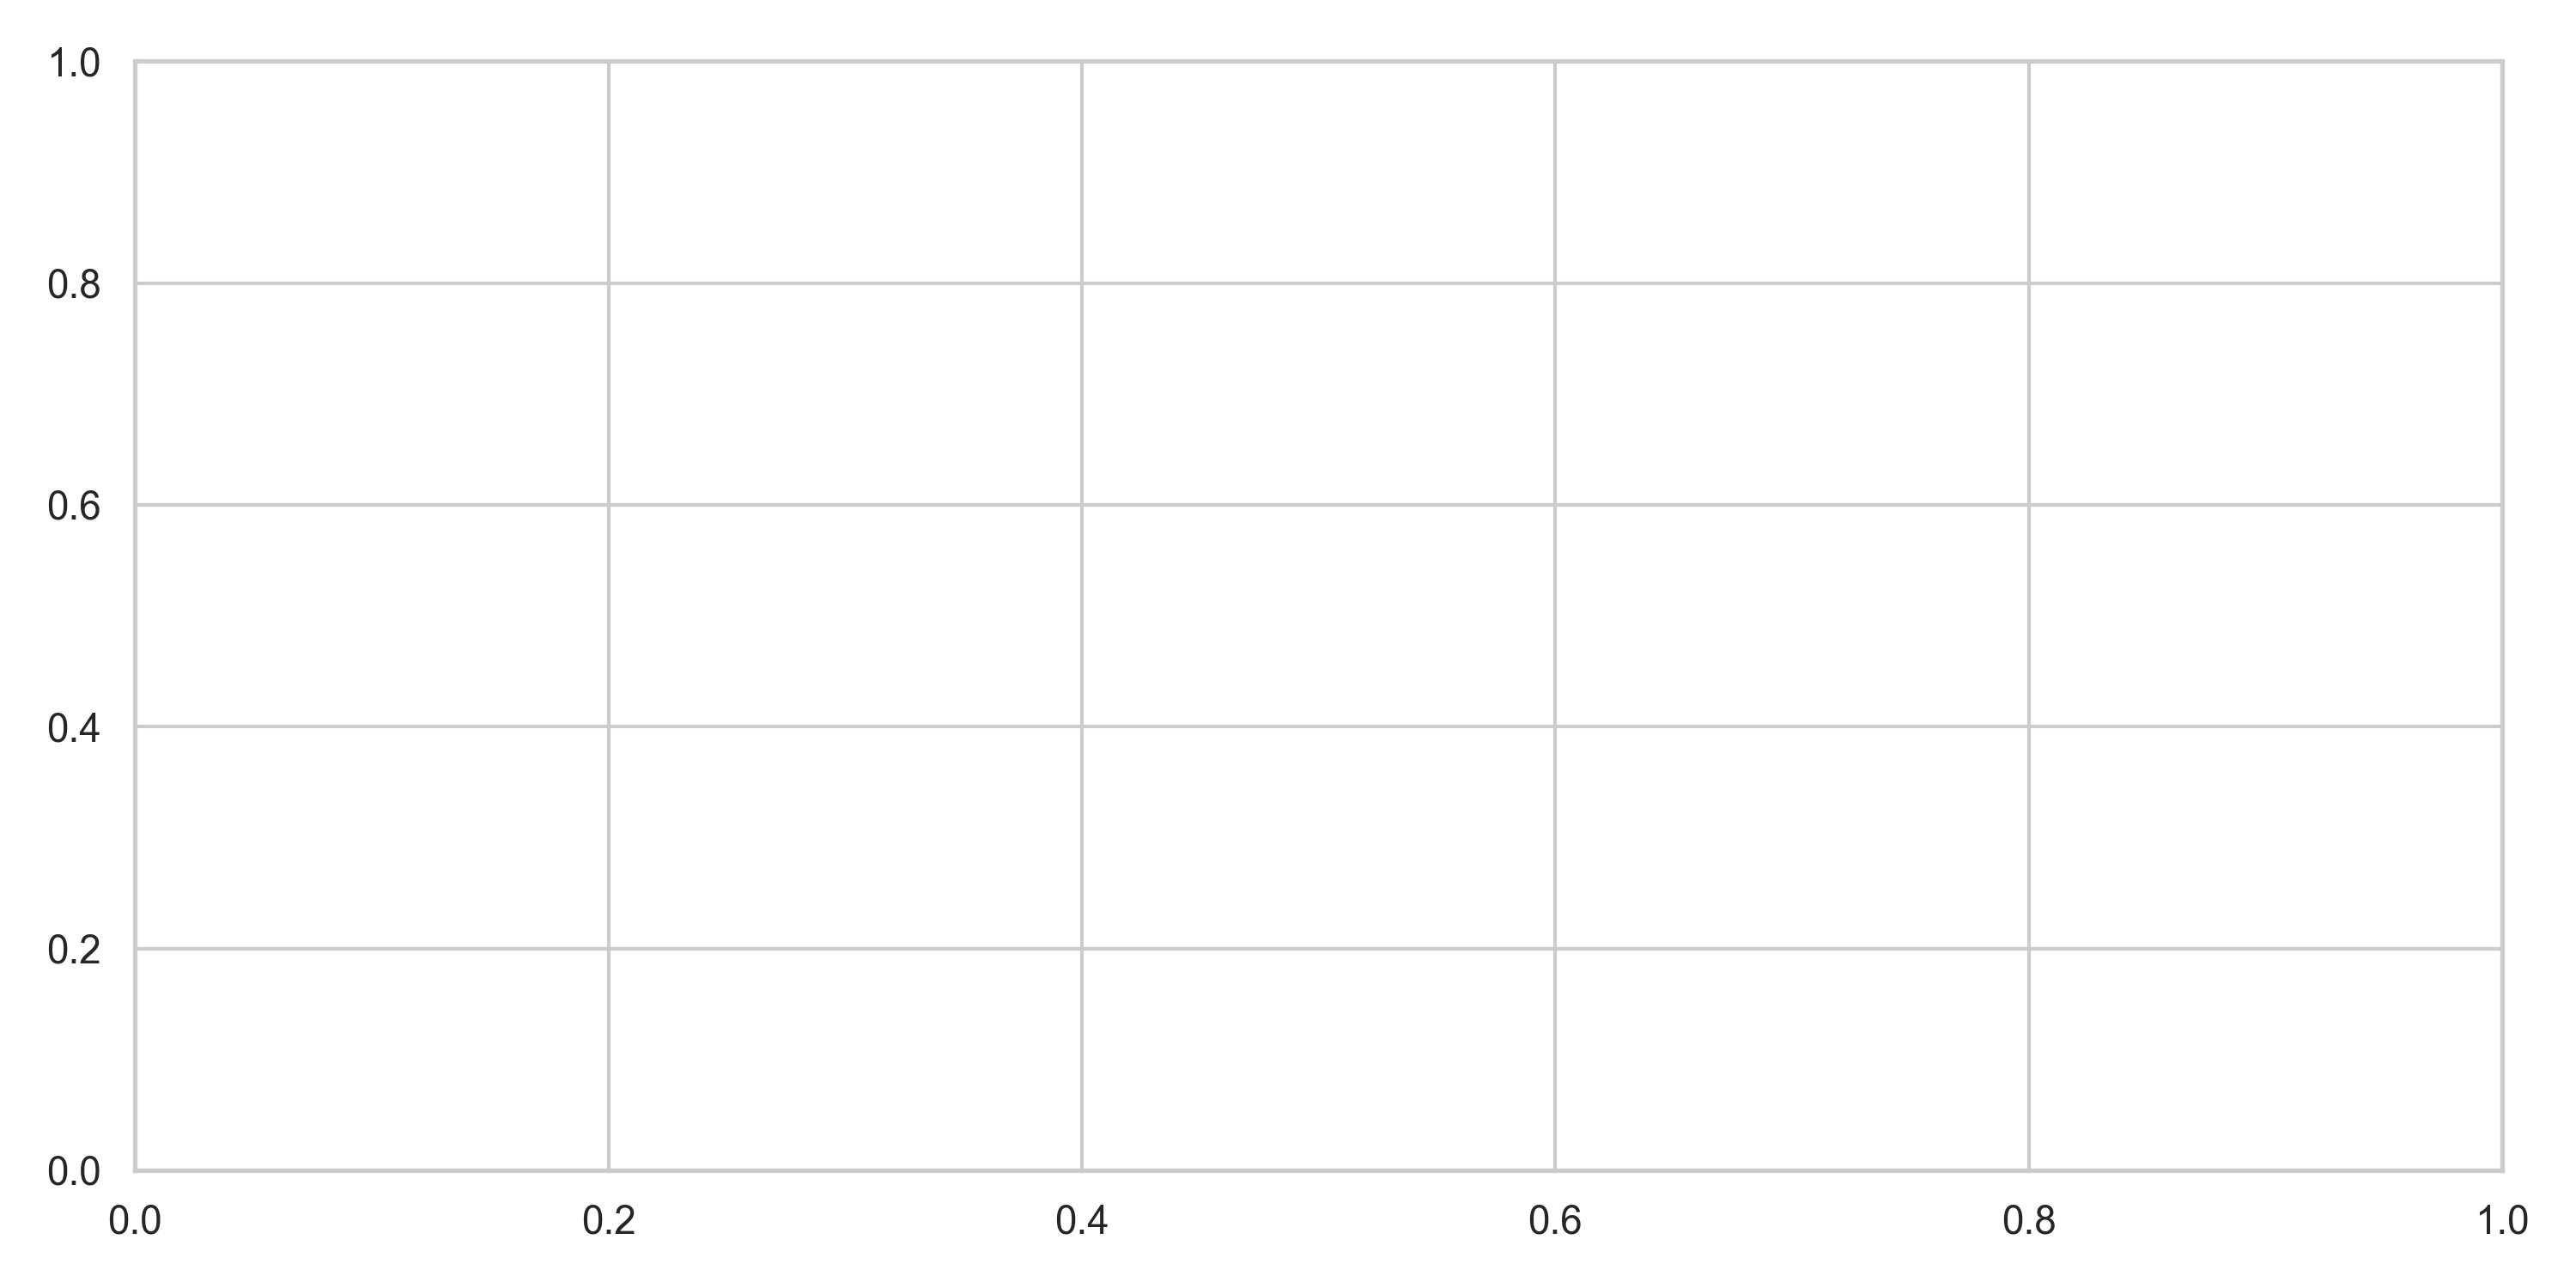
\includegraphics[width=.82\textwidth]{outputs/figures/sector_by_gender.png}
\caption{Sector distribution by gender (counts, all employed).}
\end{figure}

\begin{figure}[H]
\centering
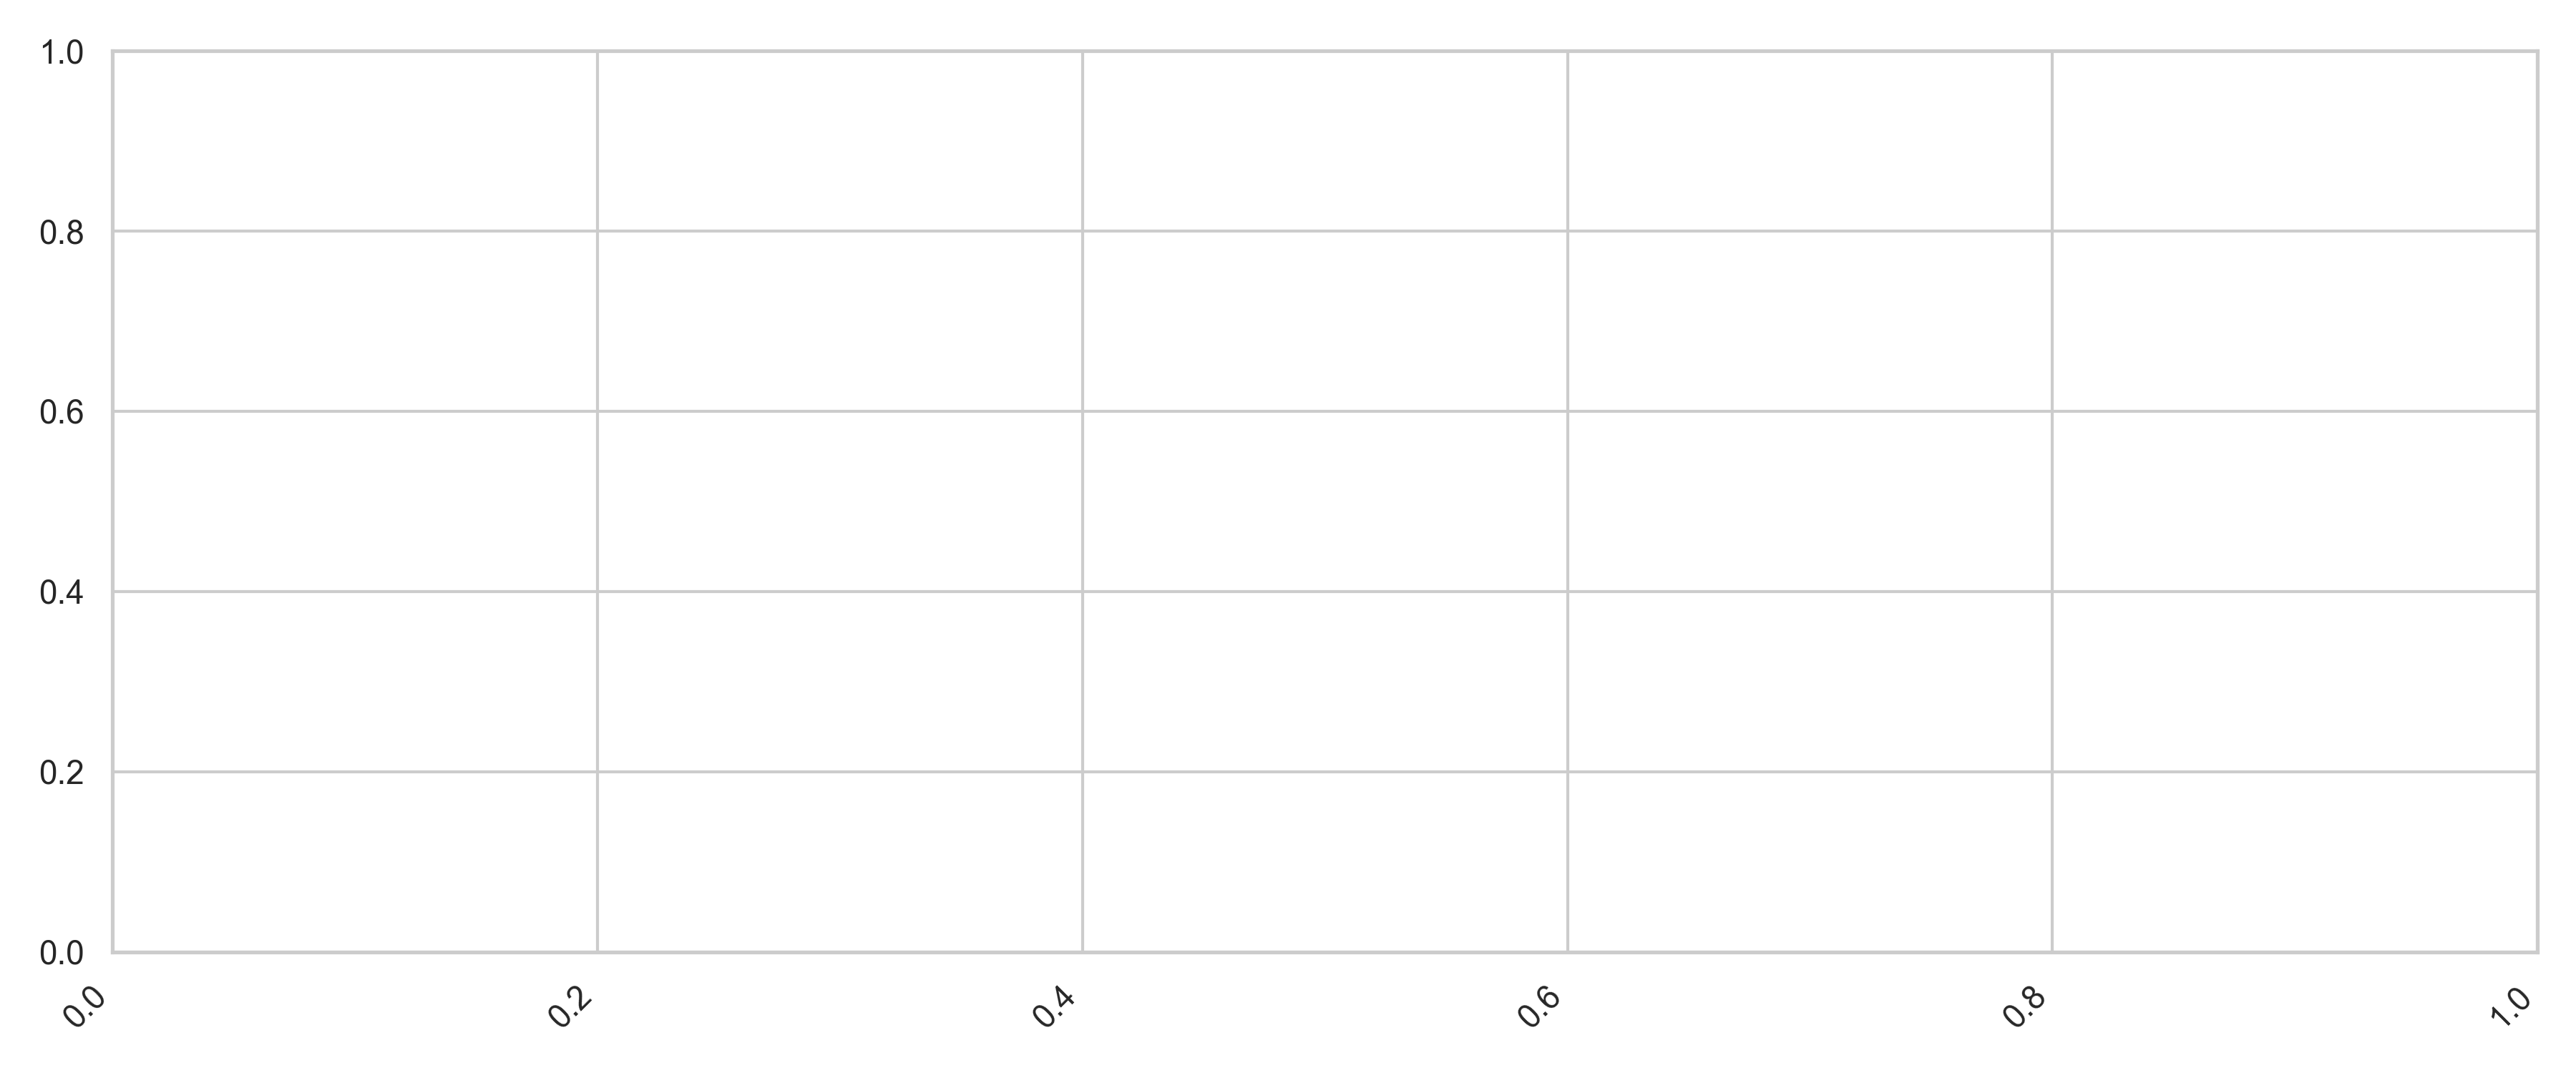
\includegraphics[width=.95\textwidth]{outputs/figures/sector_by_region.png}
\caption{Within-region sector shares, shown separately for 2024 and pooled 2021--2023.}
\end{figure}

\subsection{Q2: Disability Status and Labour-force Status}
Table: \texttt{outputs/tables/q2\_chi2\_summary.csv}.

\begin{figure}[H]
\centering
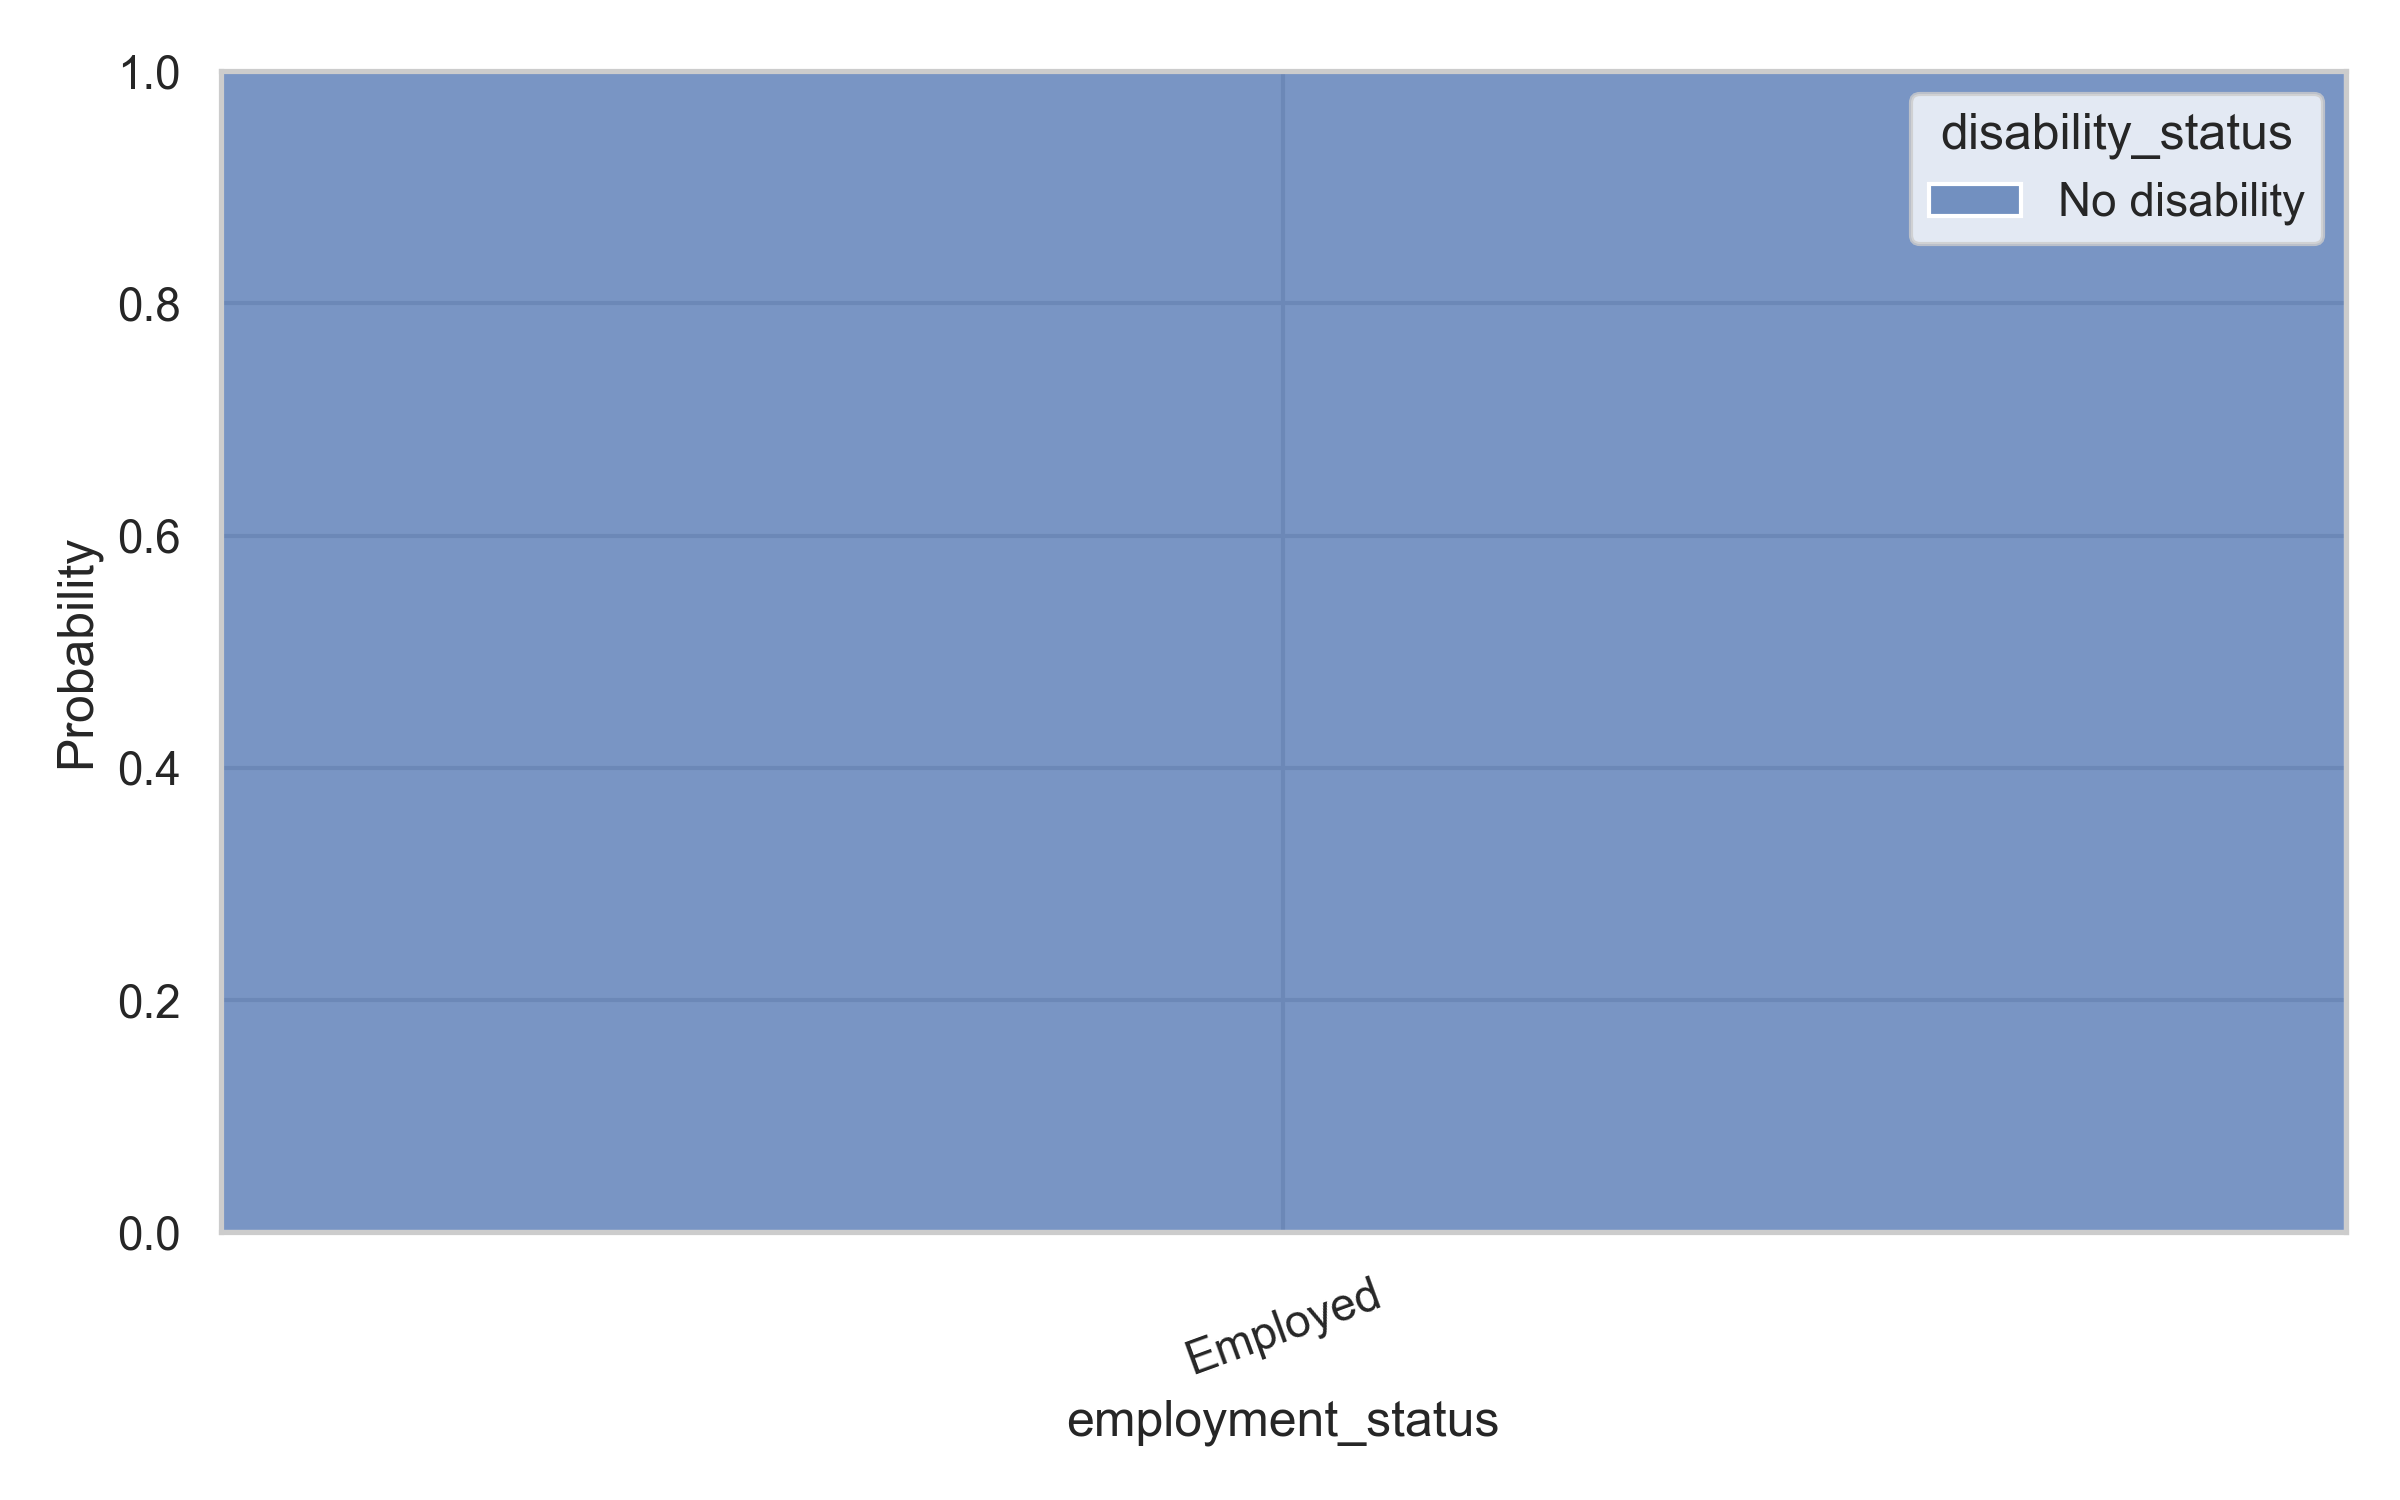
\includegraphics[width=.95\textwidth]{outputs/figures/employment_by_disability_stacked.png}
\caption{Employment-status composition by disability status, by period.}
\end{figure}

\subsection{Q3: Marital Status and Income}
Table: \texttt{outputs/tables/q3\_anova\_income.csv}.

\begin{figure}[H]
\centering
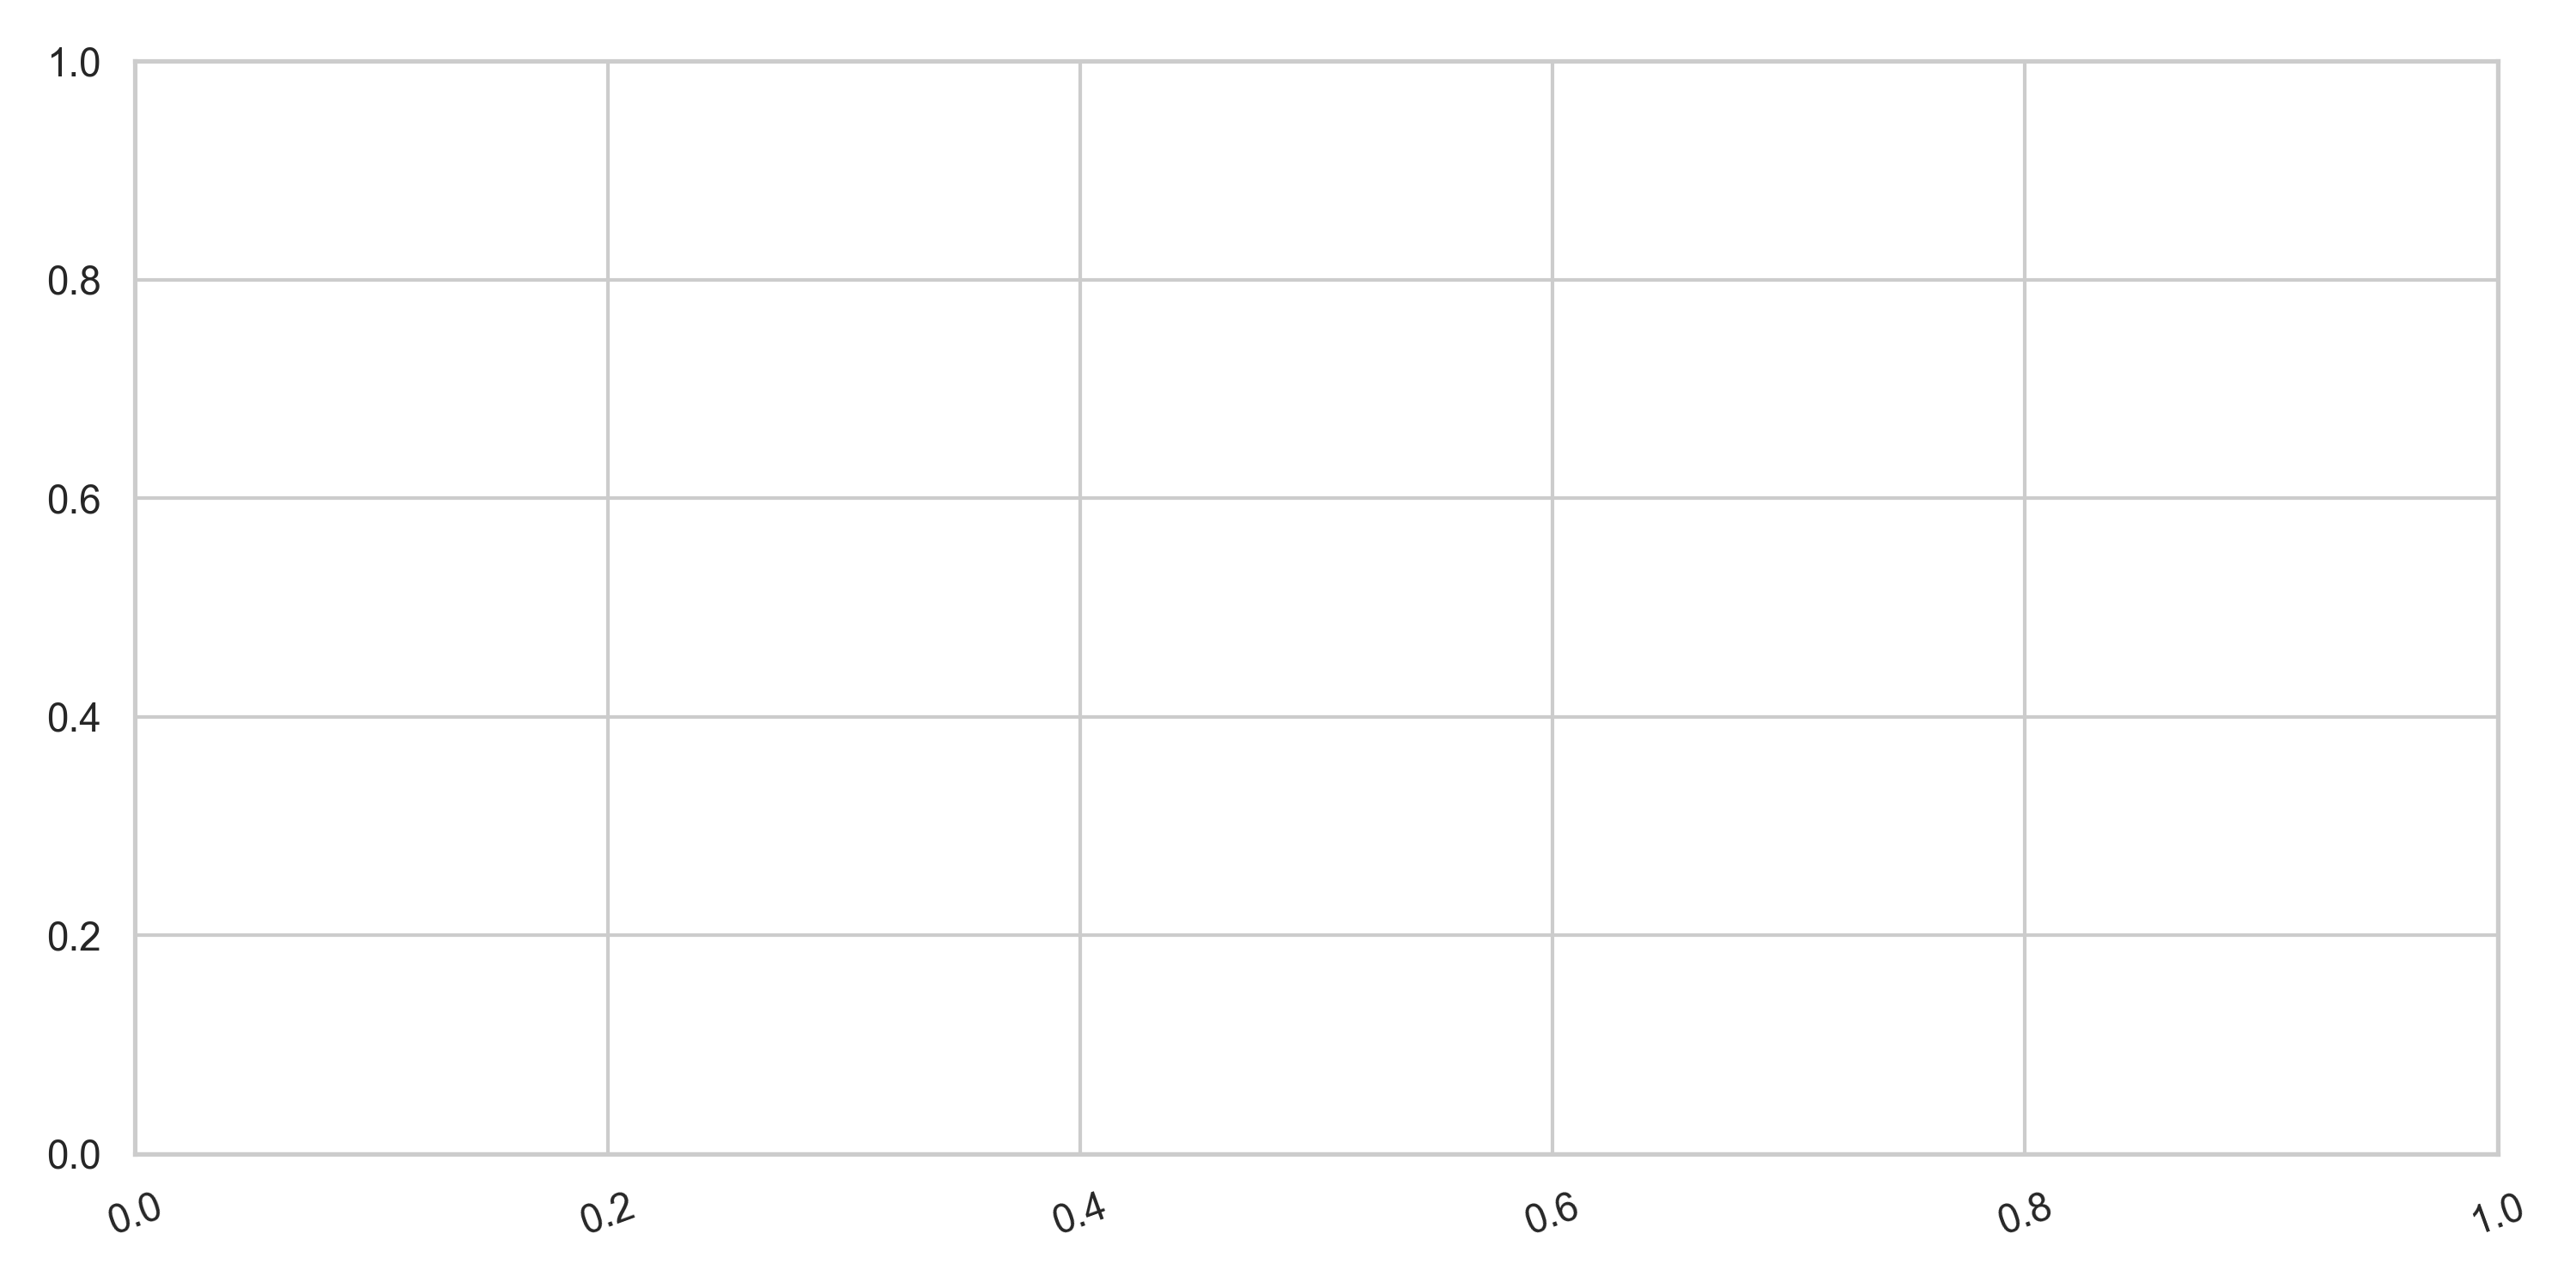
\includegraphics[width=.9\textwidth]{outputs/figures/income_by_marital.png}
\caption{Income distribution by marital status (violin + quartiles).}
\end{figure}

\begin{figure}[H]
\centering
\includegraphics[width=.9\textwidth]{outputs/figures/income_by_marital_mean_ci.png}
\caption{Mean monthly income by marital status with 95\% confidence intervals.}
\end{figure}

\subsection{Q4: Age Group and Paid Working Hours}
Table: \texttt{outputs/tables/q4\_anova\_hours.csv}.

\begin{figure}[H]
\centering
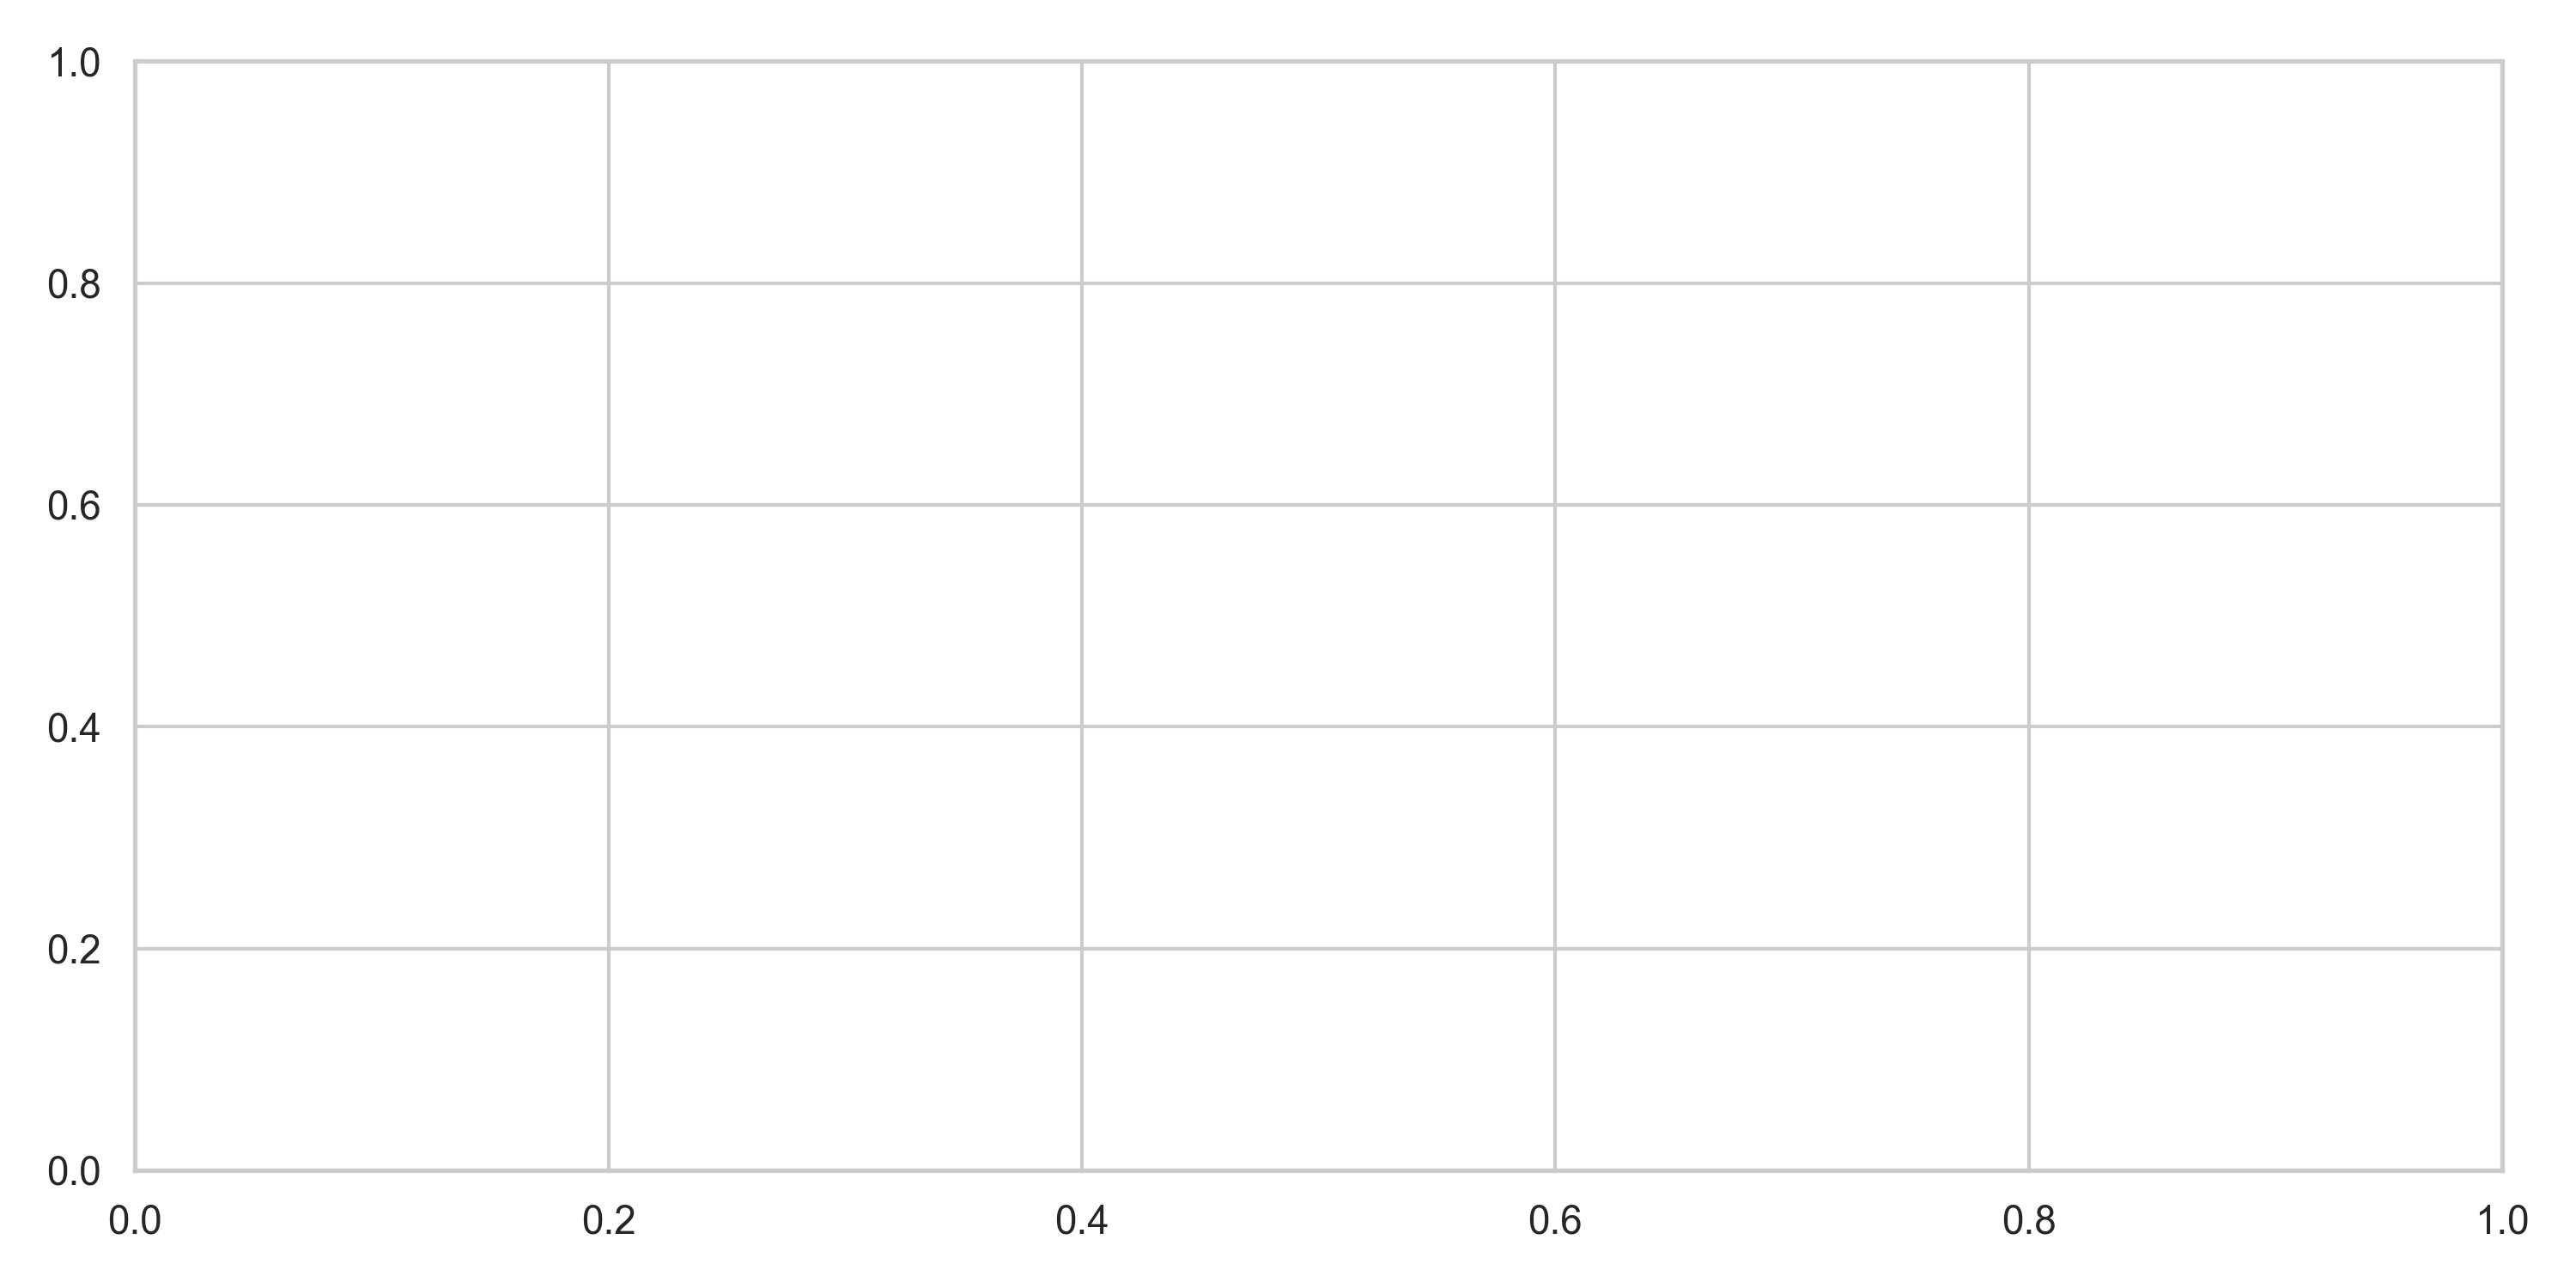
\includegraphics[width=.85\textwidth]{outputs/figures/hours_by_agegroup_ci.png}
\caption{Mean weekly paid work hours by age group with 95\% confidence intervals.}
\end{figure}

\subsection{Q5: Unpaid Domestic Work and Paid Work Hours}
Tables: \texttt{outputs/tables/q5\_regression\_summary.csv}, \texttt{q5\_regression\_*.txt}.

\begin{figure}[H]
\centering
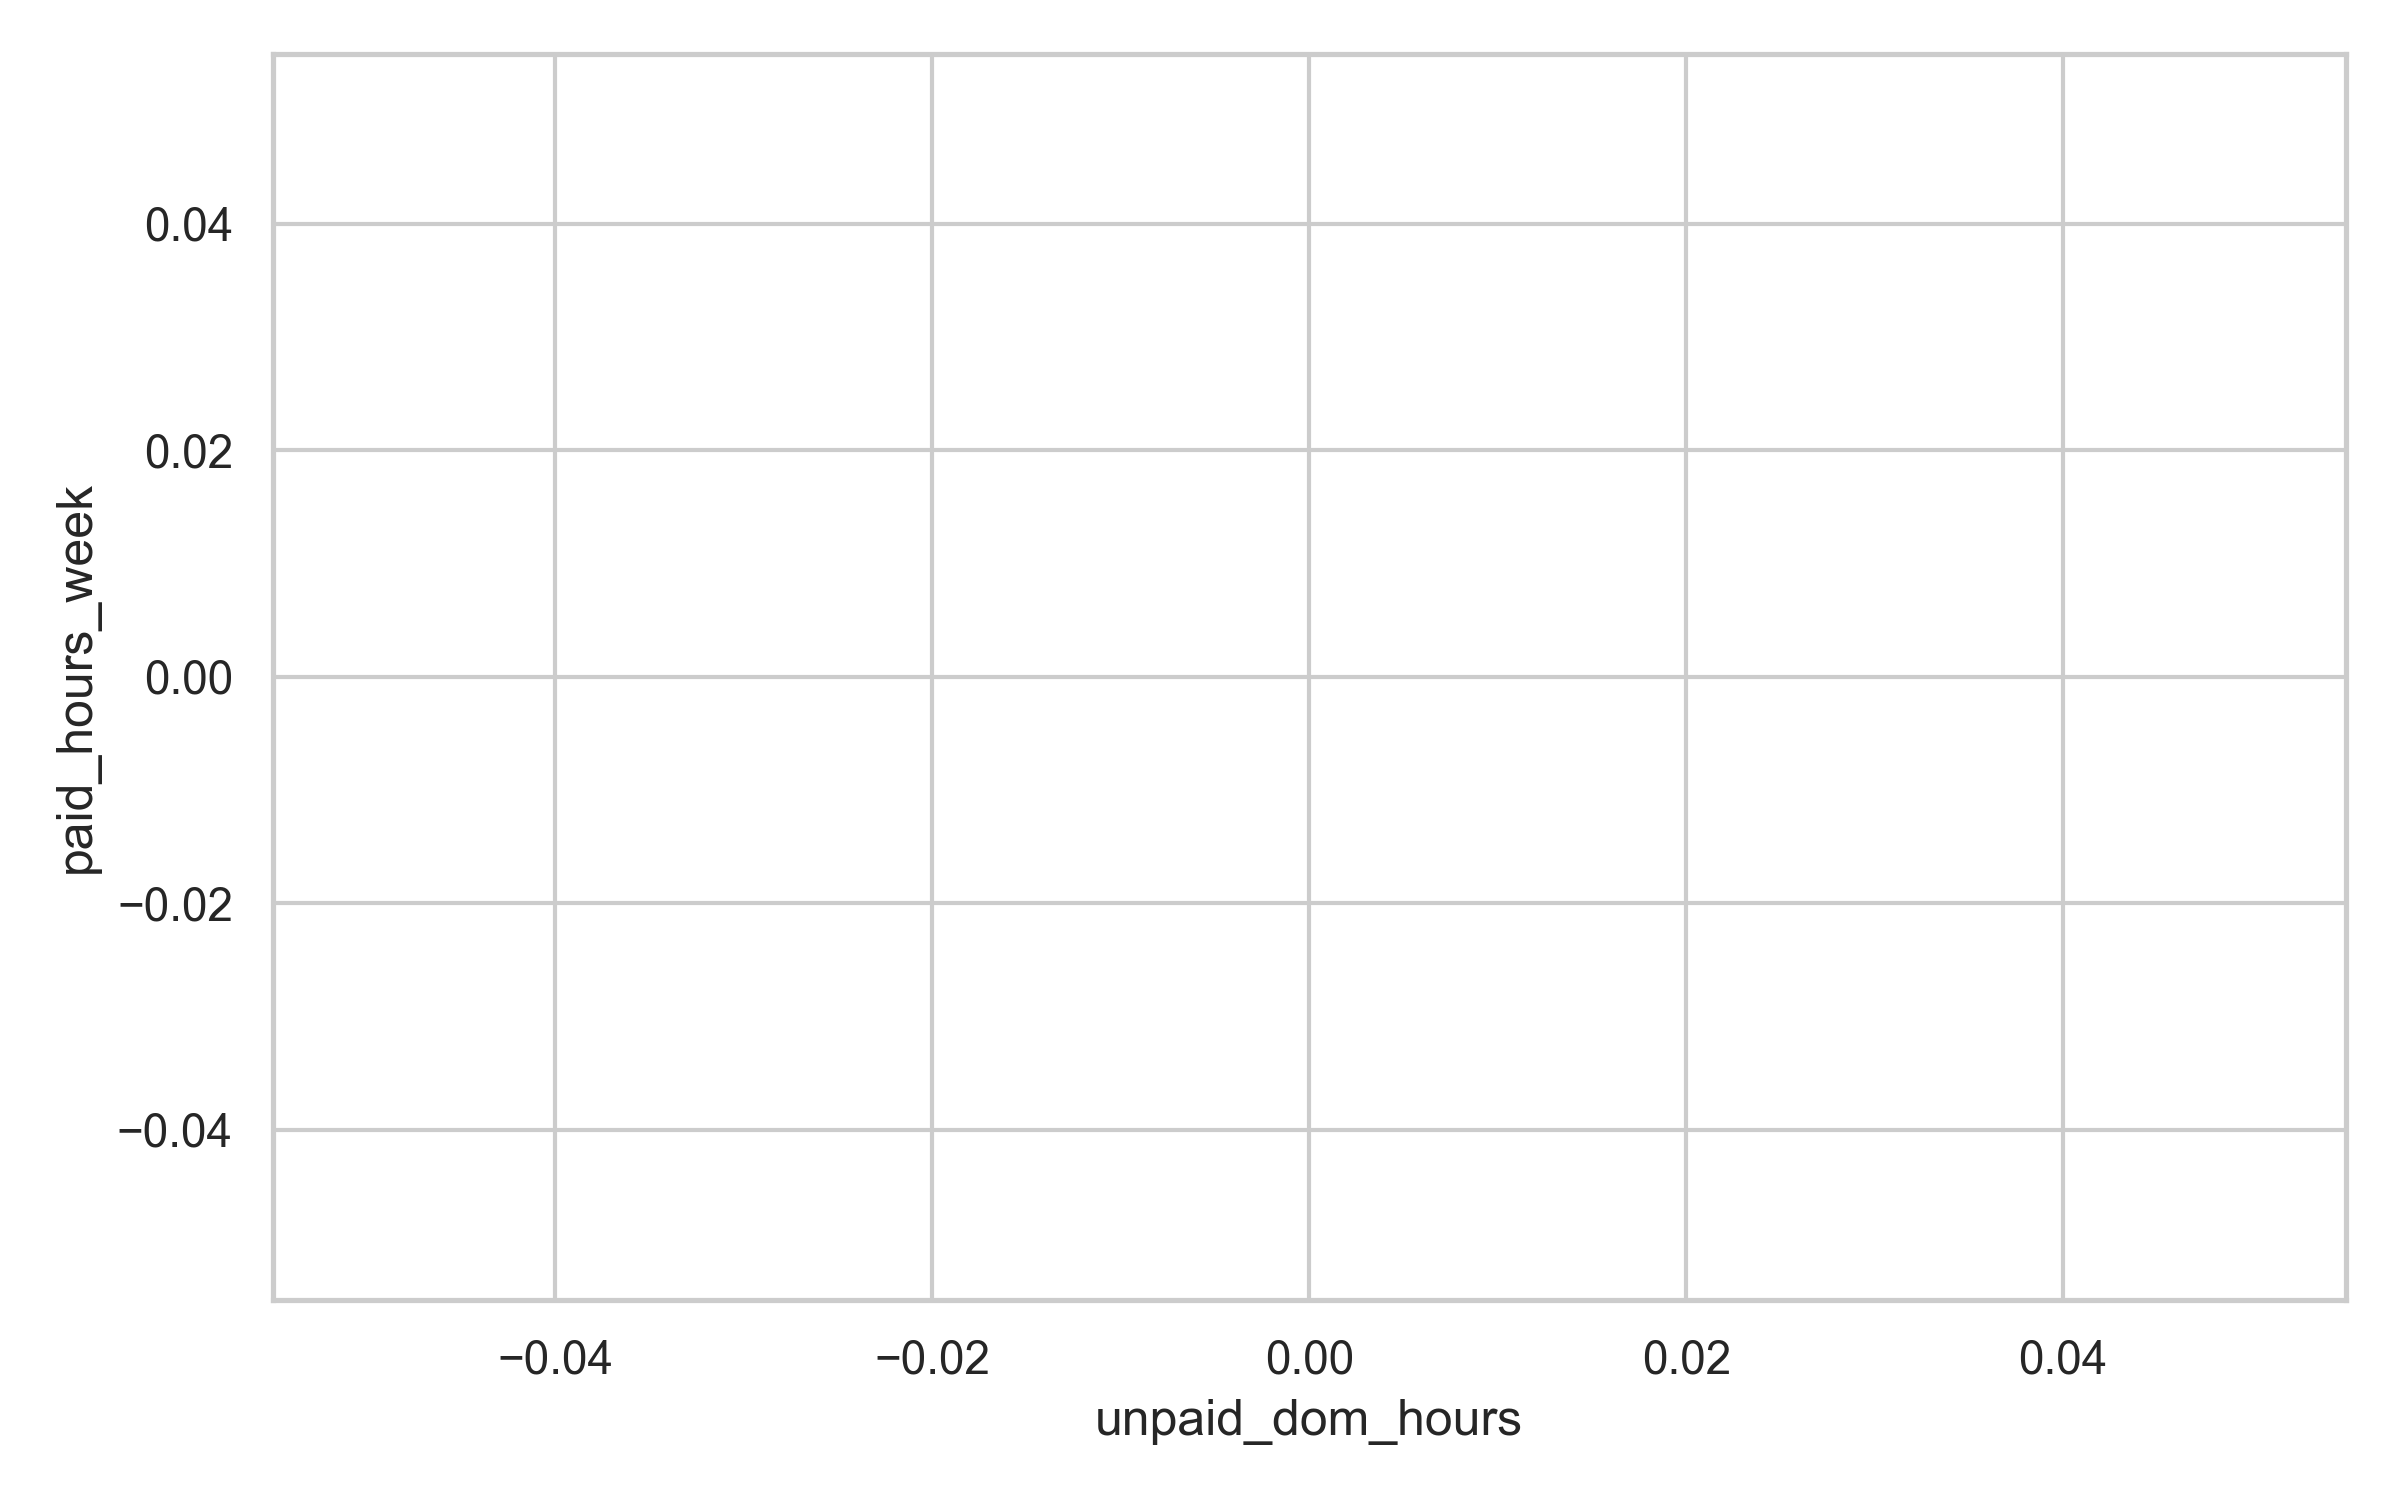
\includegraphics[width=.82\textwidth]{outputs/figures/paid_vs_unpaid_hours_reg.png}
\caption{Scatter and fitted line: unpaid domestic hours vs paid work hours.}
\end{figure}

\section{Interpretation Guidance}
When discussing findings, compare the direction and magnitude of relationships across periods (2024 vs 2021--2023), not only p-values. Report practical significance and uncertainty intervals where relevant.

\section{Limitations}
\begin{itemize}
    \item Category recodes depend on questionnaire coding consistency across years.
    \item Nonresponse and measurement error may affect income/hours variables.
    \item Complex sampling design and weighting details should be verified for inferential robustness.
\end{itemize}

\section{Reproducibility}
Run:
\begin{verbatim}
python src/lfs_analysis.py
\end{verbatim}
Then compile this report after figures/tables are generated.

\end{document}
